\chapter{Theoretical Background}

\section{Context and Motivation}

Traditionally, visual navigation research primarily relies on image-based approaches focused on drone navigation. These approaches are often limited in scalability, typically constrained to small areas or shorter flights. However, practical UAV applications may demand navigation across larger scales, even spanning hundreds of kilometers in GPS-denied scenarios. 

UAVs require stable and distinctive reference points to navigate independently over large distances without GPS. Urban areas, towns, and villages inherently exhibit different morphological structures. Recognizing these structures from high altitudes and converting them into valid reference points is the central challenge addressed in this research.

\section{Urban Morphology and Spatial Order}

Urban morphology is the study of human settlements, their structure, and the process of their formation and transformation \cite{Kropf_2017}. The spatial layout of settlements can be broadly classified into planned (often grid-like) and organic (irregular) patterns \cite{smith2007}. Urban form significantly influences how easily identifiable a settlement is, both visually and computationally.

Louf and Barthelemy \cite{remi_2014} developed a quantitative method for classifying cities by their street network "fingerprints." These fingerprints are distributions of urban block\footnote{In this context, a block is the smallest area delimited by roads} shapes and sizes - Figure \ref{fig:blocks}. Such classification can clearly distinguish North American cities (primarily grid-based patterns) from European cities (usually organic patterns). Therefore, if a UAV detects a city pattern not fitting the typical class for a region, it can reliably identify that city (e.g., Vancouver, as noted in \cite{remi_2014}).

\begin{figure}[!htb]
    \centering
    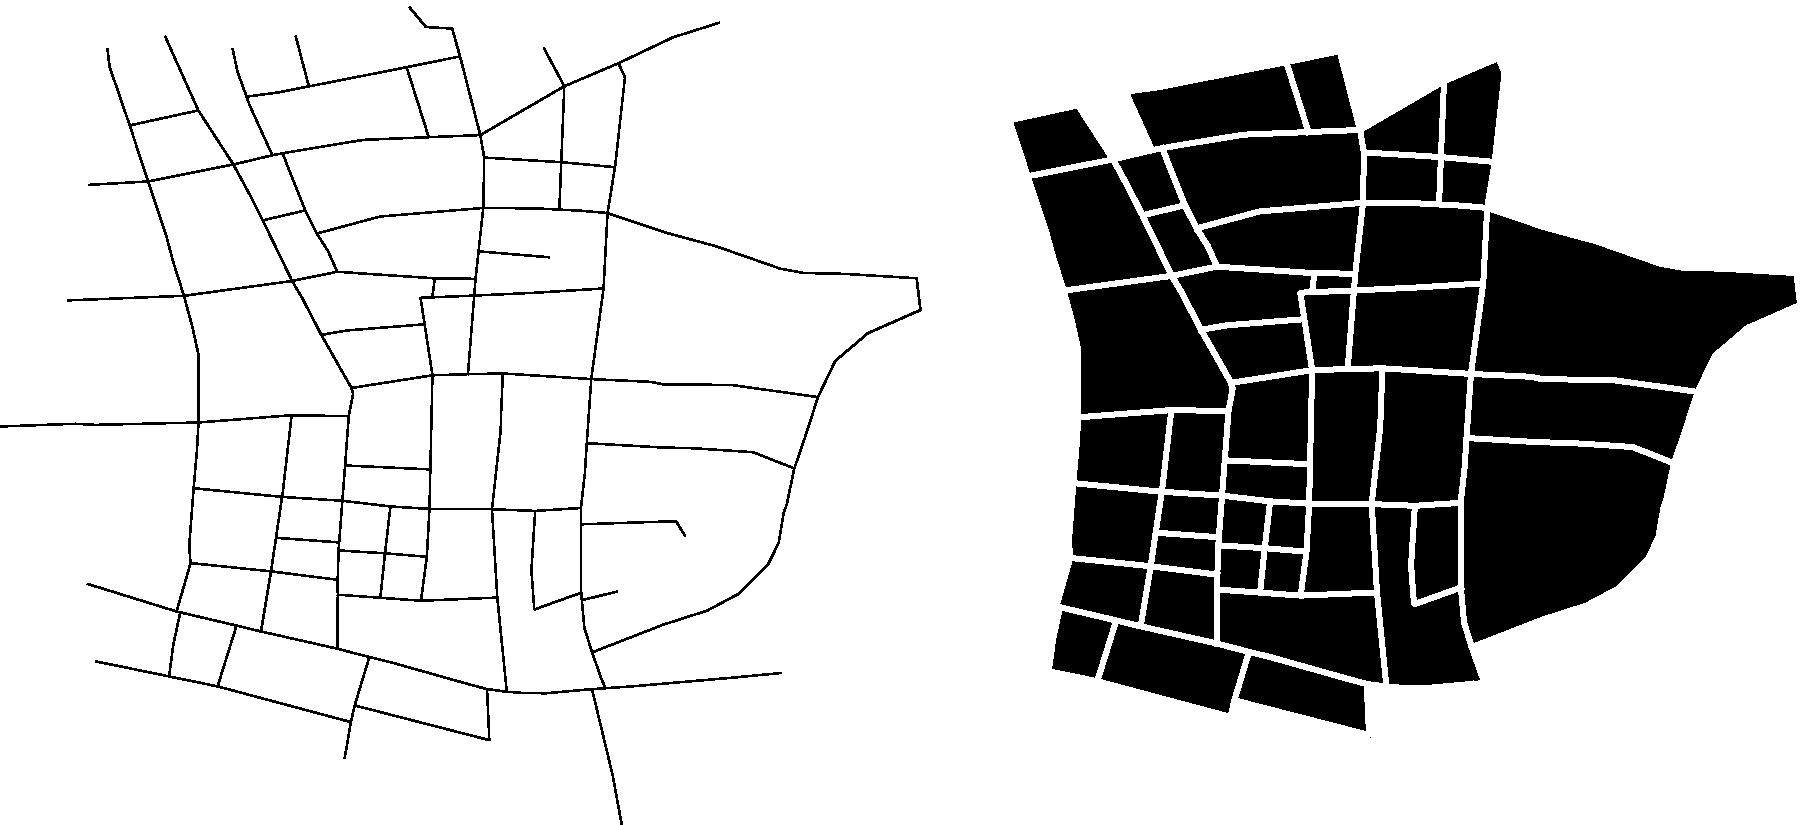
\includegraphics[width=0.8\textwidth]{Figures/figure_1.pdf}
    \caption{From the street network to blocks. Example of a street pattern taken in the neighbourhood of Shibuya in Tokyo (Japan) and the corresponding set of blocks. Note that the block representation does not take dead-ends into account \cite{remi_2014}}
    \label{fig:blocks}
\end{figure}

Geoff Boeing introduced methods for quantifying urban structure through orientation entropy and street pattern metrics \cite{Boeing_2019}. Boeing's key contribution includes the normalized orientation-order indicator $\varphi$, which measures how orderly a city's street network is compared to a perfect grid. Cities that significantly deviate from neighboring settlements' street orientation become useful reference points. Even when cities are similar in orientation-order values, the detailed distribution of their street orientations (polar histograms) may provide additional discriminative power.

\section{Machine Vision for UAV Navigation}

Machine (computer) vision is a critical component of visual navigation systems. The effectiveness of CV techniques for recognizing ground-based features depends on multiple parameters, including sensor types, camera optics, flight altitudes, speeds, viewing angles, fields of view (FoV), image resolutions, and environmental conditions. 

Standard CV methods, such as ORB\cite{ORB} (Oriented FAST and Rotated BRIEF) and SIFT\cite{SIFT} (Scale-Invariant Feature Transform), focus on extracting visual features from images, usually edges, corners, contours, and textures. These methods are robust across variations in camera perspective, illumination, and scale; thus, they and ones alike are widely used in visual navigation domain\cite{drones8070313} - see Figure \ref{fig: drones}, and can be used for further settlement classification validation.

\begin{figure}[!htb]
    \centering
    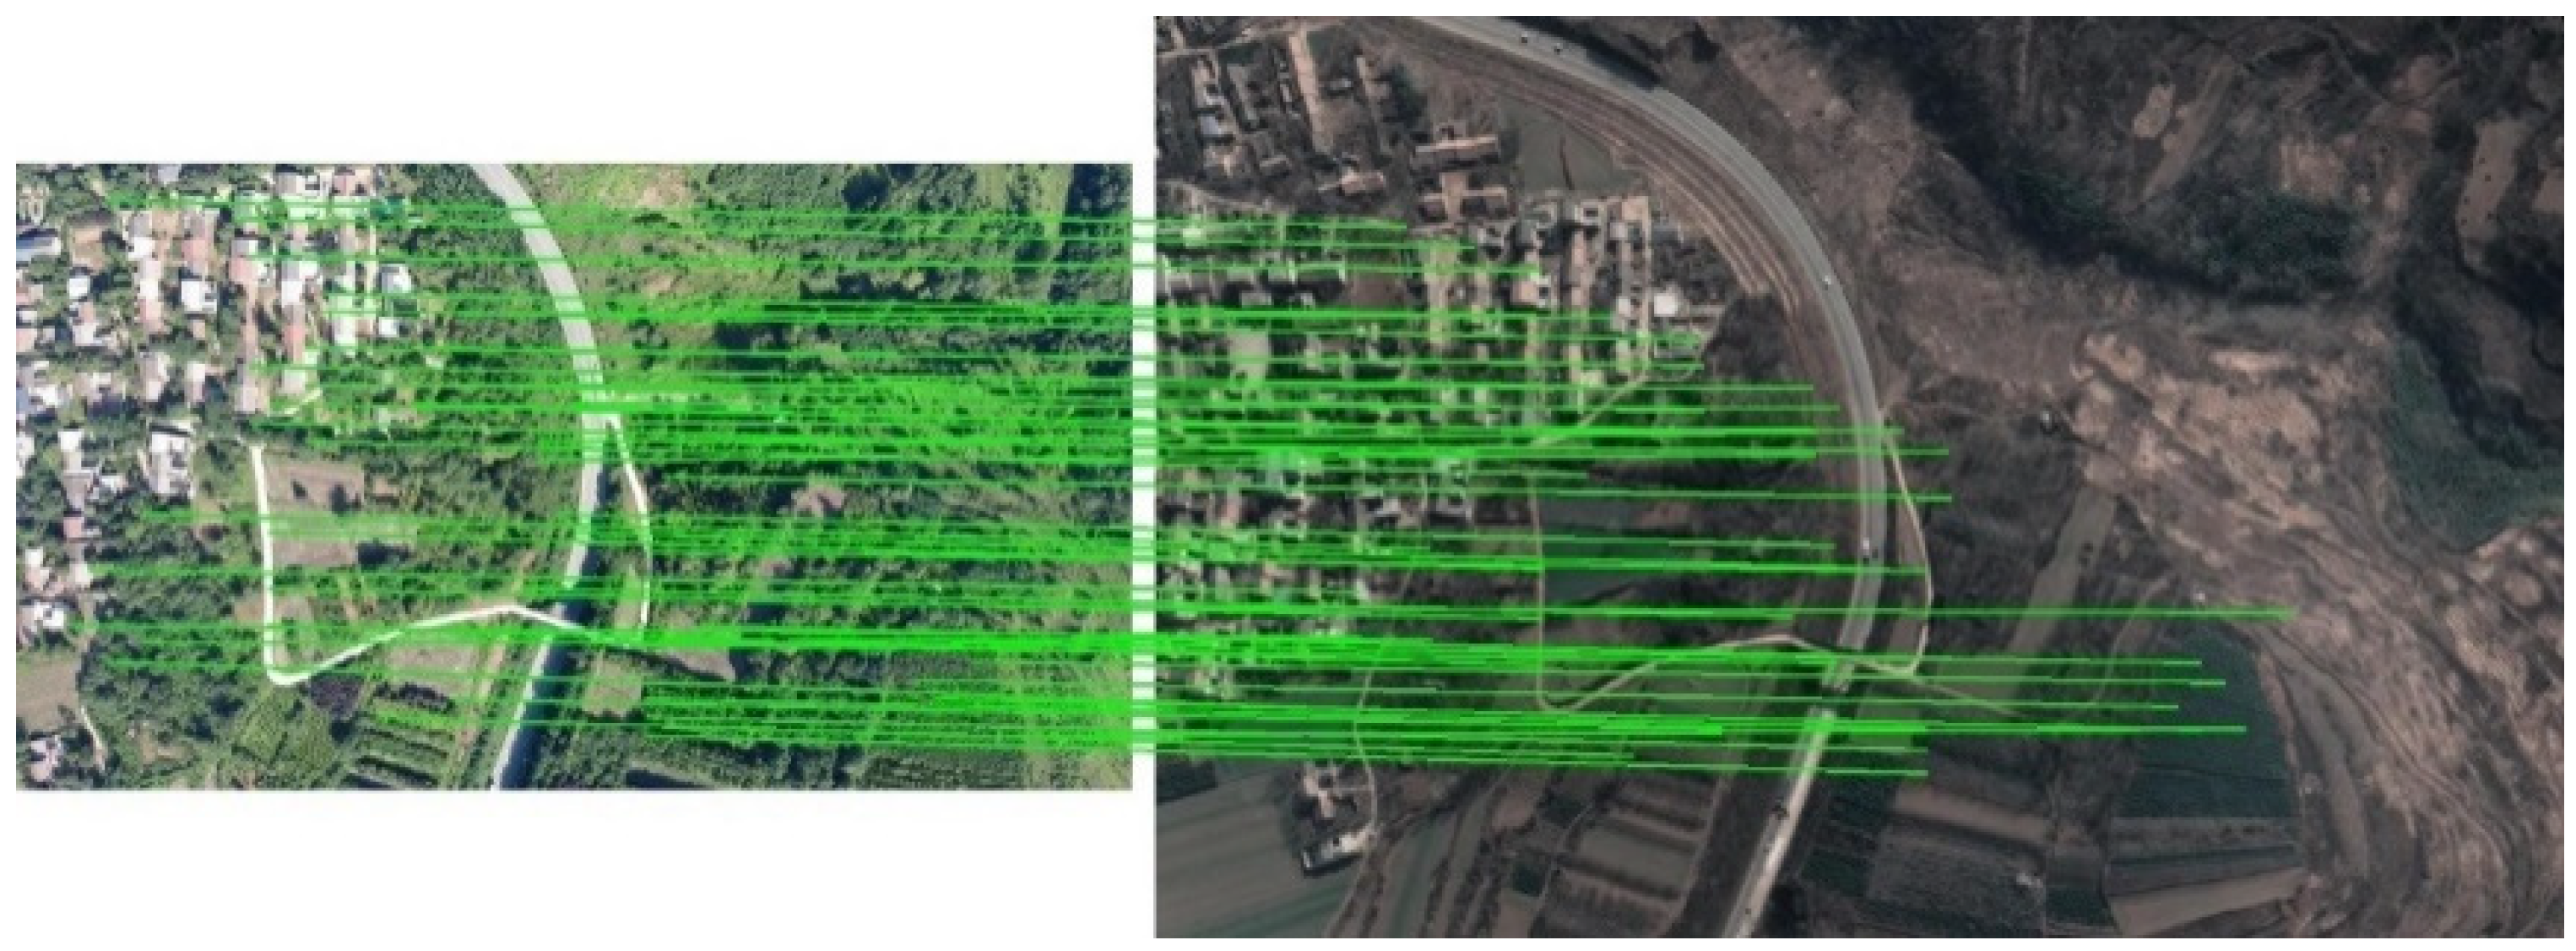
\includegraphics[width=0.8\textwidth]{Figures/drones8070313.png}
    \caption{The matching result of SuperPoint + SuperGlue. The green lines depict the extracted feature correspondences between the aerial and satellite images using SuperPoint + SuperGlue \cite{drones8070313} - ORB descriptor is used for feature extraction.}
    \label{fig:drones}
\end{figure}

However, from a high-altitude bird's-eye perspective, the visual information primarily available to UAVs consists of streets' contours and urban layouts. This contour-based information strongly correlates with street network data, which can be extracted from publicly available sources such as OpenStreetMap (OSM)\cite{OpenStreetMap}. 

\section{From Street Networks to Machine Vision}

The streets' contours directly impact the visual distinctiveness of settlements from the bird's-eye view. Specific arrangements yield more reliable and identifiable visual features. To demonstrate that we made two visualizations - maps of Lviv, Ukraine, and its Sykhiv district, we can see how the quality of the street contours is affected by the scale of the map - i.e., altitude - Figure \ref{fig:lviv_map} and Figure \ref{fig:lviv_sykhiv_map}.
% lviv_map.png lviv_sykhiv_map.png

\begin{figure}[!htb]
    \begin{minipage}{0.5\textwidth}
        \centering
        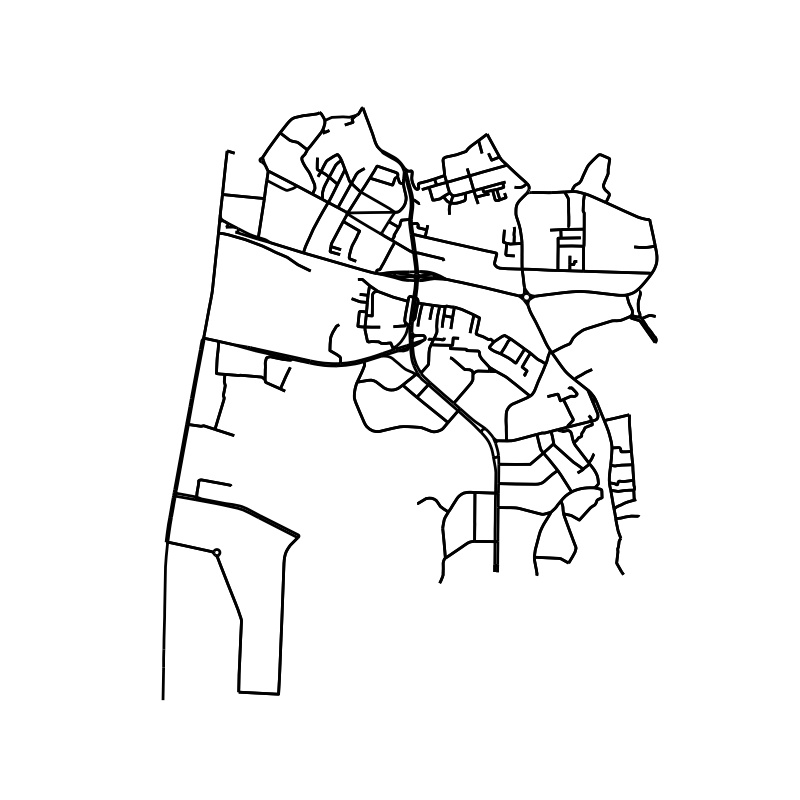
\includegraphics[width=1\linewidth]{Figures/lviv_sykhiv_map.png}
        \captionsetup{justification=justified, width=0.9\linewidth}
        \caption{Sykhiv district, Lviv, Lviv Oblast, Ukraine.}
        \label{fig:lviv_sykhiv_map}
    \end{minipage}\hfill
    \begin{minipage}{0.5\textwidth}
        \centering
        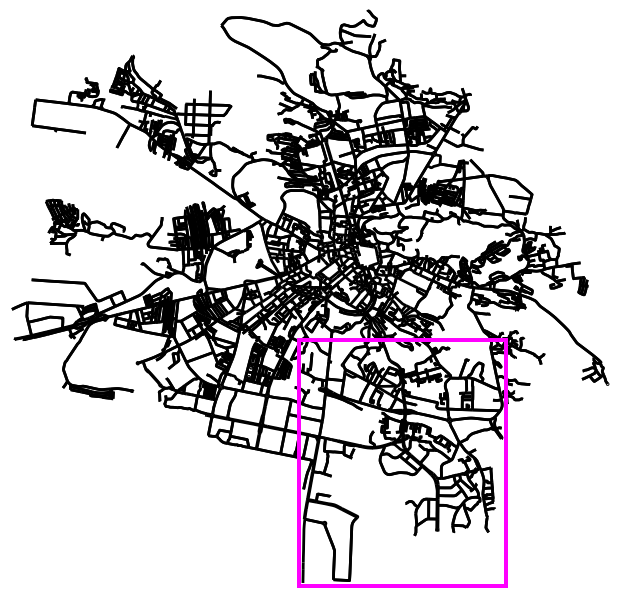
\includegraphics[width=1\linewidth]{Figures/lviv_map.png}
        \captionsetup{justification=justified, width=0.95\linewidth}
        \caption{Lviv, Lviv Oblast, Ukraine. Magenta rectangle indicates the Sykhiv district.}
        \label{fig:lviv_map}
    \end{minipage}
\end{figure}


There are many researches on this topic, such as \citetitle{li2020road} by \citet{li2020road}, that focus on road segmentation - Figure \ref{fig:li2020road}, intersections extraction from aerial images - Figure \ref{fig:li2020road2}, and drone localization based on derived data.

\begin{figure}[!htb]
    \centering
    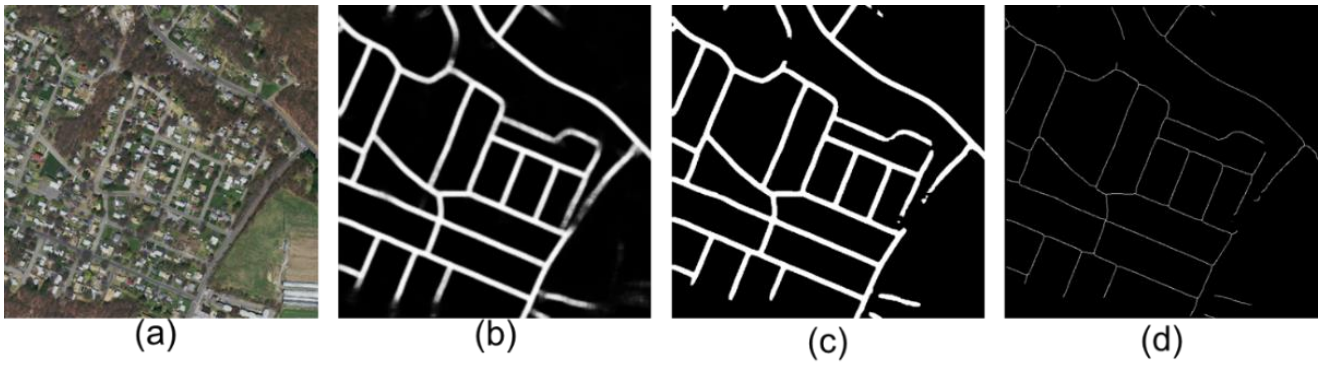
\includegraphics[width=0.8\textwidth]{Figures/li2020road1.png}
    \caption{Road intersections detection and description. (a)Query aerial image. (b)Road segmentation result. (c)Binary road image. (d) Skeletonized road image \cite{li2020road}}
    \label{fig:li2020road}
\end{figure}

\begin{figure}[!htb]

    \centering

    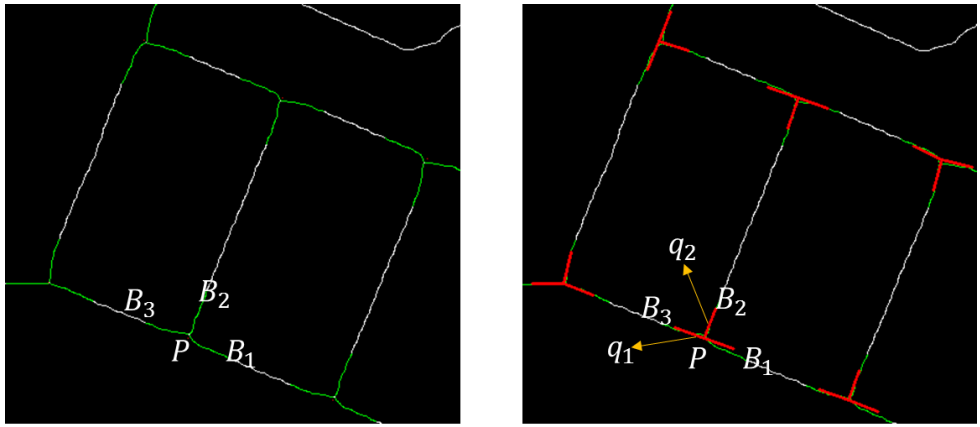
\includegraphics[width=0.8\textwidth]{Figures/li2020road2.png}

    \caption{Road intersection branches segmentation and tangents estimation\dots \cite{li2020road}}

    \label{fig:li2020road2}

\end{figure}

Settlements can, therefore, be categorized based on how their street patterns stand out visually. For example, a highly regular grid may appear repetitive to computer vision algorithms, making it challenging to recognize uniquely. Irregular or uniquely organized patterns may provide distinctive visual signatures, making them valuable reference points.

We propose using standard computer vision descriptors, such as ORB and SIFT, to objectively validate the subjective classifications of visual distinctiveness derived from spatial metrics. This validation step bridges the conceptual gap, thus confirming that geospatially distinctive areas are also suitable as navigational reference points for UAVs.

\section{Research Approach and Hypotheses}

This research builds upon the methodologies of Louf and Barthelemy, and Boeing, creating a new analytical layer that is relevant to visual navigation. We also transform available street network data into simplified contour-based maps suitable for classification validation using computer vision analysis.

The research will compare and categorize settlements at multiple scales:

\begin{itemize}

    \item Small villages

    \item Larger villages or city districts

    \item Small cities

    \item Large cities

\end{itemize}


We transform available geospatial data into new labeled data points that represent how suitable each location is as a reference point for UAV visual navigation. Each data point will be assigned one of the following labels, creating a clear and understandable taxonomy:


\begin{itemize}
    \item \textbf{Class A (Excellent)} - Areas highly suitable as reference points due to distinctive and easily recognizable urban layouts from a bird's-eye view. These typically feature unique street patterns or configurations that significantly stand out.
    \item \textbf{Class B (Good)} - Areas suitable as reliable reference points with clear visual distinctiveness, though less prominent than Class A. They contain recognizable but less unique urban configurations.
    \item \textbf{Class C (Normal)} - Areas that may serve as reference points but provide limited distinctive visual features, making them less reliable for visual navigation unless combined with additional contextual data.
    \item \textbf{Class D (Poor)} - Areas with minimal or no distinctive urban layout characteristics. They are unreliable for navigation but better than nothing.
    \item \textbf{No Data} - Areas lacking sufficient geospatial data for meaningful classification or analysis.
\end{itemize}


These labels provide a clear taxonomy for systematically evaluating settlements at multiple geographic scales (villages, districts, small cities, and large cities). This subjective labeling is subsequently validated using computer vision feature descriptors.


Thus, the research hypotheses are:

\begin{enumerate}

    \item Integration of Boeing's normalized orientation-order ($\varphi$) and polar histograms with Louf and Barthelemy's urban fingerprints is more effective at classification than using them separately, resulting in reference points for long-range UAV navigation.

    \item Urban map features correlate with the performance of computer vision descriptors (ORB and SIFT) on contour-based maps, making them valuable for practical UAV visual navigation.

\end{enumerate}

% \section{Research Aims and Hypotheses}



% Based on the theoretical concepts described, this research aims to:



% \begin{itemize}

%     \item Use urban morphology methods (Louf's fingerprints, Boeing's entropy metrics) to identify visually distinct settlements at multiple scales.

%     \item Quantify the correlation between urban street networks and CV feature extraction from bird's-eye-view images.

%     \item Classify settlements into different scales (e.g., villages, towns, city districts, cities) and evaluate their suitability for UAV visual navigation.

% \end{itemize}



% To achieve these aims, the following hypotheses guide this study:



% \begin{enumerate}

%     \item Urban fingerprints (Louf and Barthelemy's method) can effectively distinguish visually unique settlements that serve as reliable UAV navigation reference points.

%     \item Boeing's entropy-based orientation metrics can identify local anomalies useful for UAV navigation.

%     \item The urban street network layout significantly influences the extraction and robustness of visual descriptors (e.g., ORB, SIFT) from contour-based aerial imagery.

% \end{enumerate}



% Testing these hypotheses through rigorous data analysis will demonstrate the practical utility of urban morphological analyses and street network data for UAV navigation, ultimately enabling scalable, robust, and reliable GPS-independent UAV navigation systems.

% \chapter{Theoretical Background }



% Traditionally, visual navigation research primarily relies on image-based approaches focused on drone navigation at relatively short distances. This study challenges the abovementioned limited perception by highlighting the value of geospatially distinctive\footnote{The degree of uniqueness and recognizability of urban regions based on spatial characteristics.} regions independent of direct image processing techniques.



% This study integrates concepts from urban morphology, street network analysis, street network orientation, configuration and entropy, and urban form typologies. The methodology builds on established theories and frameworks by \citet{remi_2014} and \citet{Boeing_2019}, expanding these concepts to use visual distinctiveness for practical navigation applications. Using them, we measure scene attractiveness\footnote{Suitability of a geospatial area as a visual navigation reference point}, thus complementing previous efforts and creating new opportunities in the long-range flight planning field.



% \section{Urban Morphology and Spatial Order}



% Urban morphology is the study of human settlements, their structure, and the process of their formation and transformation \cite{Kropf_2017}. They may be systematically planned, typically exhibiting grid-like patterns, or emerge organically, reflecting irregular, spontaneous development responding to local constraints \cite{smith2007}. These morphological patterns significantly affect a city's spatial distinctiveness, which this research aims to quantify and leverage for visual navigation.



% Louf and Barthelemy classified cities into four distinct groups based on the shapes and areas of their urban blocks, thus introducing the concept of urban fingerprints. In this context, a block is the smallest area delimited by roads - see Figure \ref{fig:blocks}. This typological classification provides a systematic and quantitative basis for recognizing distinctive urban patterns. Cities sharing similar block shapes, areas, and distributions form identifiable groups.



% \begin{figure}[!htb]

%     \centering

%     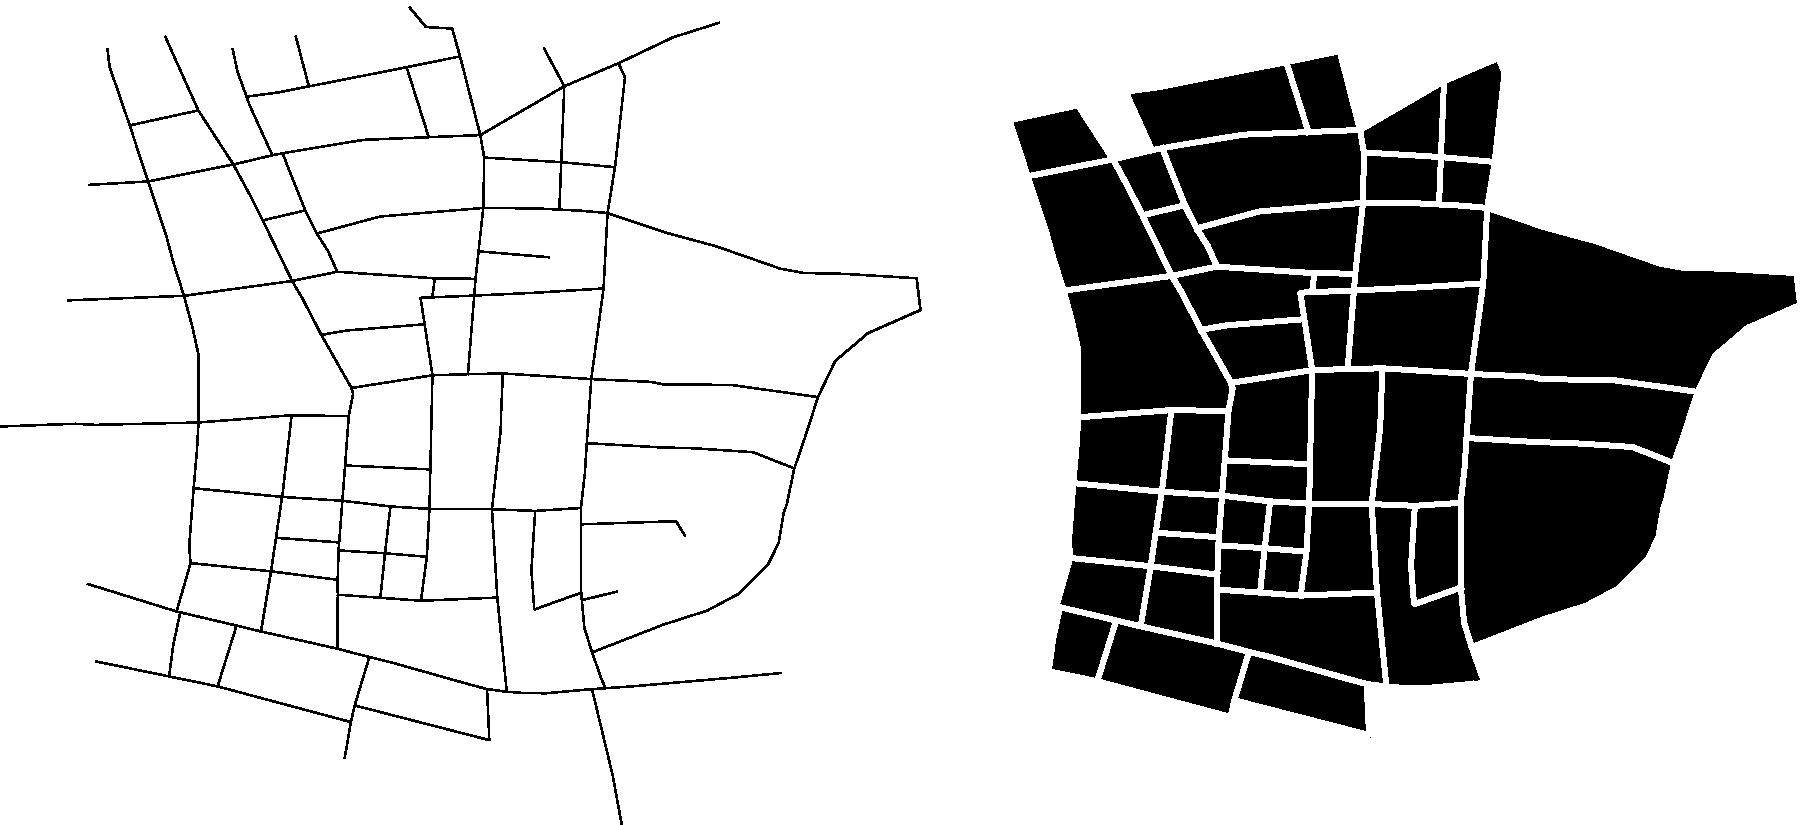
\includegraphics[width=0.8\textwidth]{Figures/figure_1.pdf}

%     \caption{From the street network to blocks. Example

%     of a street pattern taken in the neighbourhood of Shibuya

%     in Tokyo (Japan) and the corresponding set of blocks. Note

%     that the block representation does not take dead-ends into

%     account \cite{remi_2014}}

%     \label{fig:blocks}

% \end{figure}



% Geoff Boeing used street network entropy to quantify urban spatial order and disorder and classified cities into clusters based on normalized measures of orientation-order, median street segment length, average node degree, and network's average circuity. Street orientation entropy assesses the variability in street segment orientations within urban networks. Low entropy indicates systematic, grid-like urban forms, while high entropy represents irregular, complex networks typical of historically or organically evolved cities \cite{Boeing_2019}.



% Combining these concepts, we introduce a new basis for cities' classification. Urban fingerprints offer a quantifiable typology to classify urban forms systematically. Street networks' orientation, configuration, entropy, and blocks' area and shape factor form the concept of scene attractiveness, which underpins the identification of visually distinctive navigation points. Using new data, one can make a framework for visual navigation planning at broader geographic scales, suitable for varied distances and contexts beyond conventional visual navigation scenarios, particularly relevant in GPS-denied environments.

